\documentclass[tikz,border=5pt]{standalone}
\usetikzlibrary{patterns} % 加载斜线阴影库
\begin{document}
	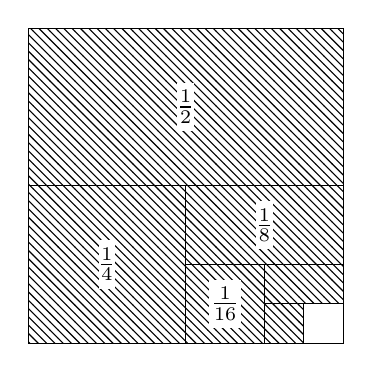
\begin{tikzpicture}[scale=2]
		% 绘制大正方形边框
		\draw (0,0) rectangle (2,2);
		
		% 标注 1/2 的区域(上半部分)
		\filldraw[pattern=north west lines] (0,1) rectangle (2,2);
		\filldraw[white] (0.95,1.35) rectangle (1.05,1.65);
		\node at (1,1.5) {$\frac{1}{2}$};
		
		% 标注 1/4 的区域(左下部分)
		\filldraw[pattern=north west lines] (0,0) rectangle (1,1);
		\filldraw[white] (0.45,0.35) rectangle (0.55,0.65);
		\node at (0.5,0.5) {$\frac{1}{4}$};
		
		% 标注 1/8 的区域(右下上半部分)
		\filldraw[pattern=north west lines] (1,0.5) rectangle (2,1);
		\filldraw[white] (1.45,0.6) rectangle (1.55,0.9);
		\node at (1.5,0.75) {$\frac{1}{8}$};
		
		% 标注 1/16 的区域(右下左半部分)
		\filldraw[pattern=north west lines] (1,0) rectangle (1.5,0.5);
		\filldraw[white] (1.15,0.1) rectangle (1.35,0.4);
		\node at (1.25,0.25) {$\frac{1}{16}$};
		
		% 更小的斜线填充区域
		\filldraw[pattern=north west lines] (1.5,0.25) rectangle (2,0.5);
		
		% 空白小正方形
		\filldraw[pattern=north west lines] (1.5,0) rectangle (1.75,0.25);
		
	\end{tikzpicture}
\end{document}
